\documentclass[tikz, border=10pt]{standalone}
\usepackage{tikz}
\usepackage{amsmath,amssymb}
\usetikzlibrary{arrows.meta, positioning, calc, shapes, fit}

\begin{document}

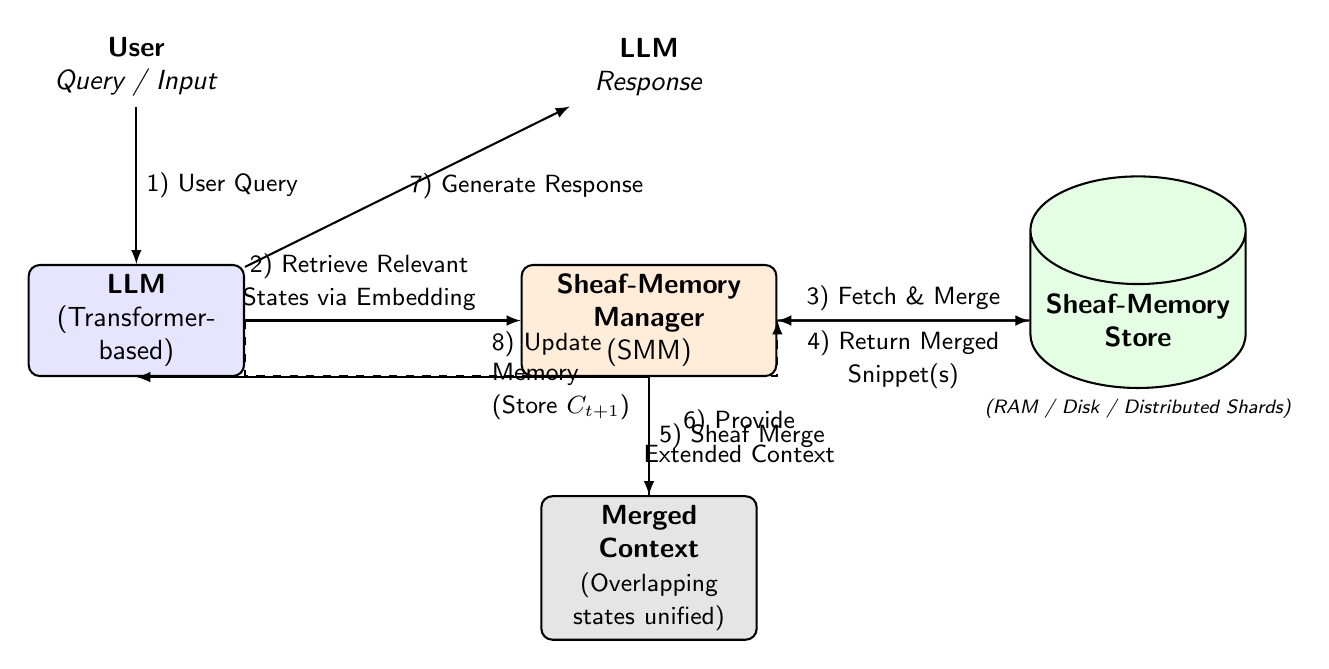
\begin{tikzpicture}[
    font=\sffamily,
    node distance=2.5cm,
    >=latex,
    line width=0.75pt,
    every node/.style={align=center},
    box/.style={rectangle, draw, rounded corners, minimum width=2.0cm, minimum height=1.0cm},
    db/.style={cylinder, draw, shape aspect=0.5, minimum height=1.5cm,
               cylinder uses custom fill, cylinder body fill=white, shape border rotate=90}
]

% ----------------------
% Nodes
% ----------------------

% LLM node
\node[box, fill=blue!10, text width=2.5cm] (llm) {\textbf{LLM} \\ (Transformer-based)};

% SMM node
\node[box, fill=orange!15, text width=3.0cm, right=3.5cm of llm] (smm) {\textbf{Sheaf-Memory Manager}\\(SMM)};

% Memory store
\node[db, fill=green!10, text width=2.5cm, right=3.2cm of smm, 
    label=below:{\scriptsize \textit{(RAM / Disk / Distributed Shards)}}] (mem) {\textbf{Sheaf-Memory Store}};

% User Query
\node[above=2.0cm of llm, align=center, text width=2.5cm] (user) {\textbf{User}\\ \textit{Query / Input}};

% Output / Response
\node[above=2.0cm of smm, align=center, text width=2.3cm] (resp) {\textbf{LLM}\\ \textit{Response}};

% Merged context snippet
\node[box, fill=gray!20, below=1.5cm of smm, text width=2.5cm] (merge) {\textbf{Merged Context}\\ \small(Overlapping states unified)};

% ----------------------
% Arrows
% ----------------------

% From user to LLM
\draw[->] (user) -- node[midway, right, xshift=0.0cm] {\small 1) User Query} (llm.north);

% LLM to SMM (query for context)
\draw[->] (llm) -- node[midway, above, xshift=-0.3cm] {\small 2) Retrieve Relevant\\ \small States via Embedding} (smm);

% SMM to Memory store
\draw[->] (smm) -- node[midway, above] {\small 3) Fetch \& Merge} (mem);

% Memory store back to SMM
\draw[->] (mem) -- node[midway, below] {\small 4) Return Merged\\ \small Snippet(s)} (smm);

% SMM to merged context snippet (vertical downward arrow)
\draw[->] (smm) -- node[midway, right] {\small 5) Sheaf Merge} (merge);

% Merged context snippet to LLM (arrow up)
\draw[->] (merge) |- node[pos=0.25, right, xshift=-0.2cm] {\small 6) Provide\\ \small Extended Context} (llm.south);

% LLM response arrow going upward
\draw[->] (llm) -- node[midway, right, xshift=-0.1cm] {\small 7) Generate Response} (resp);

% LLM to SMM (updating memory with new state)
\draw[->, dashed] (llm.east) |- ++(0.5, -0.7) -| node[pos=0.2, right, text width=2.2cm, align=left] {\small 8) Update Memory \\ (Store $C_{t+1}$)} (smm.east);

\end{tikzpicture}

\end{document}
